\documentclass[a4paper, 12pt]{article}
\usepackage[T2A,T1]{fontenc}
\usepackage[utf8]{inputenc}
\usepackage[english, russian]{babel}
\usepackage{graphicx}
\usepackage[hcentering, bindingoffset = 10mm, right = 15 mm, left = 15 mm, top=20mm, bottom = 20 mm]{geometry}
\usepackage{multirow}
\usepackage{lipsum}
\usepackage{amsmath, amstext}
\usepackage{siunitx}
\usepackage{subcaption}
\usepackage{wrapfig}
\usepackage{adjustbox}
\usepackage{enumerate, indentfirst, float}
\usepackage{capt-of, svg}
\usepackage{icomma}

\newenvironment{bottompar}{\par\vspace*{\fill}}{\clearpage}
 
\begin{document}
\begin{titlepage}

\newcommand{\HRule}{\rule{\linewidth}{0.5mm}} % Defines a new command for the horizontal lines, change thickness here

\center % Center everything on the page
 
%----------------------------------------------------------------------------------------
%	HEADING SECTIONS
%----------------------------------------------------------------------------------------

\textsc{\LARGE Московский \\[0.5cm] Физико-Технический Институт}\\[1,5cm] % Name of your university/college
\textsc{\Large Кафедра общей физики}\\[0.5cm] % Major heading such as course name
\textsc{\large Лабораторная работа \textnumero  3.2.4}\\[0.5cm] % Minor heading such as course title

%----------------------------------------------------------------------------------------
%	TITLE SECTION
%----------------------------------------------------------------------------------------

\HRule
\\[0.4cm]
{ \huge \bfseries Свободные колебания в электиреском контуре}
\\[0.2cm] % Title of your document
\HRule
\\[1.5cm]


 
%----------------------------------------------------------------------------------------
%	AUTHOR SECTION
%----------------------------------------------------------------------------------------

%\begin{minipage}{0.4\textwidth}
	\begin{flushleft} \large
		\emph{Студент:}\\
		Павел \textsc{Северилов} \\
		671 группа
	\end{flushleft}
%\end{minipage}


\begin{bottompar}
	\begin{center}
		
\includegraphics[width = 80 mm]{logo.jpg}
	\end{center}
	{\large \today}

\end{bottompar}
\vfill % Fill the rest of the page with whitespace

\end{titlepage}

\section{Цель работы}
Исследование свободных колебаний в колебательном контуре.

\textbf{В работе используются:} \textit{генератор импульсов, электронное реле, магазин сопротивлений, магазин емкостей, индуктивность, электронный осциллограф, универсальный мост.}


\section{Теоретическая часть}
Импульсы от генератора поступают на колебательный контур через реле (диодный тиристор D и ограничительный резистор $R_1$). Импульсы заряжают конденсатор $C$. После каждого импульса генератор откючается от колебательного контура, и в контуре возникают свободные затухающие колебания, которые можно наблюдать на осциллографе.

Схема экспериментальной установки: 
$$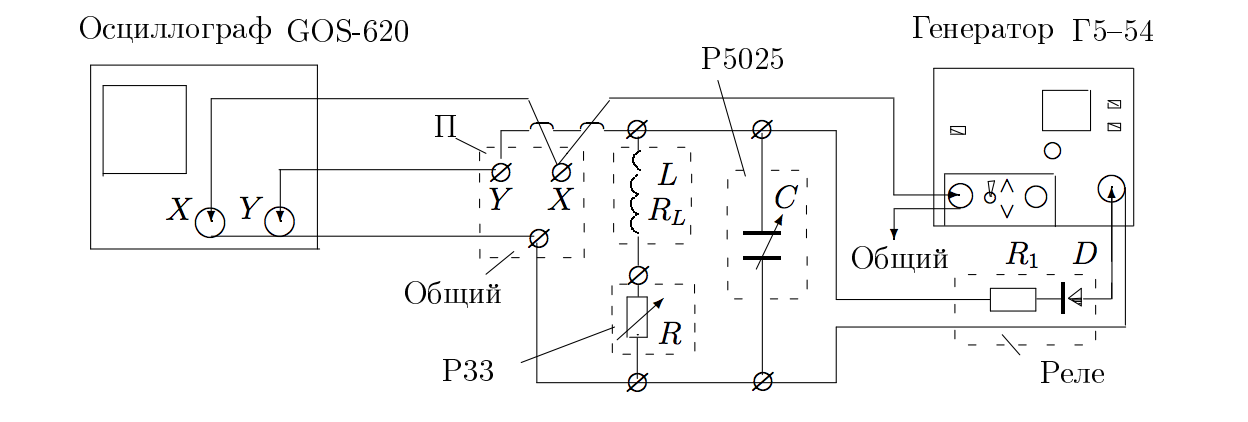
\includegraphics[scale=0.7]{scheme}$$

Здесь: $L$ -- постоянная индуктивность, $C$ и $R$ -- переменные ёмкость и сопротивление соответственно.

\section{Работа и измерения}
\begin{enumerate}
	\item Прокалибруем горизонтальную ось осциллографа по известному периоду повторения импульсов:
	\begin{itemize}
		\item подберем частоту развертки осциллографа, при которой расстояние $x_0$ между импульсами, поступающими с генератора ($T_0 = 0,01$с), занимает почти весь экран.
		\item измерим на экране расстояние $x$, которое занимают несколько полных периодов $n$.
		\item период колебаний контура $T = T_0\cfrac{x}{nx_0}$ -- эксперимент
		\item $T$ теоретический: $T = \cfrac{2\pi}{\omega_0} = 2\pi\sqrt{LC}$, $L\simeq135.4 \text{мГн}$
	\end{itemize}
	Результаты вносим в Таблицу 1.
	\begin{table}[H]
		\centering
		\begin{tabular}{|c|c|c|c|c|c|}
			\hline
			$C, \text{ мкФ}$ & $x_0$ & $x$ & $n$ & $T_{exp}, 10^{-4}\text{ с}$ & $T_{theor}, 10^{-4}\text{ с}$ \\ \hline
		0,02&	5,7&	8,6&	5&	3,270&	3,018  \\ \hline
		0,15&	5,7&	9,2&	2&	8,954&	8,070  \\ \hline
		0,25&	5,8&	8,8&	1,5&	11,560&	10,115  \\ \hline
		0,35&	5,7&	7&	1	&13,678	&12,281  \\ \hline
		0,45&	5,7&	7,8&	1&	15,509&	13,684  \\ \hline
		0,55&	5,7&	8,7&	1&	17,146&	15,263  \\ \hline
		0,65&	5,7&	9,3&	1&	18,640&	16,316  \\ \hline
		0,75&	5,7&	10,3&	1&	20,023&	18,070  \\ \hline
		\end{tabular}
		\caption{$T_{exp}$ и $T_{theor}$}
	\end{table}
	Построим график $T_{exp}=f(T_{theor})$:
	
	\begin {figure}[H]
	\begin{center}
		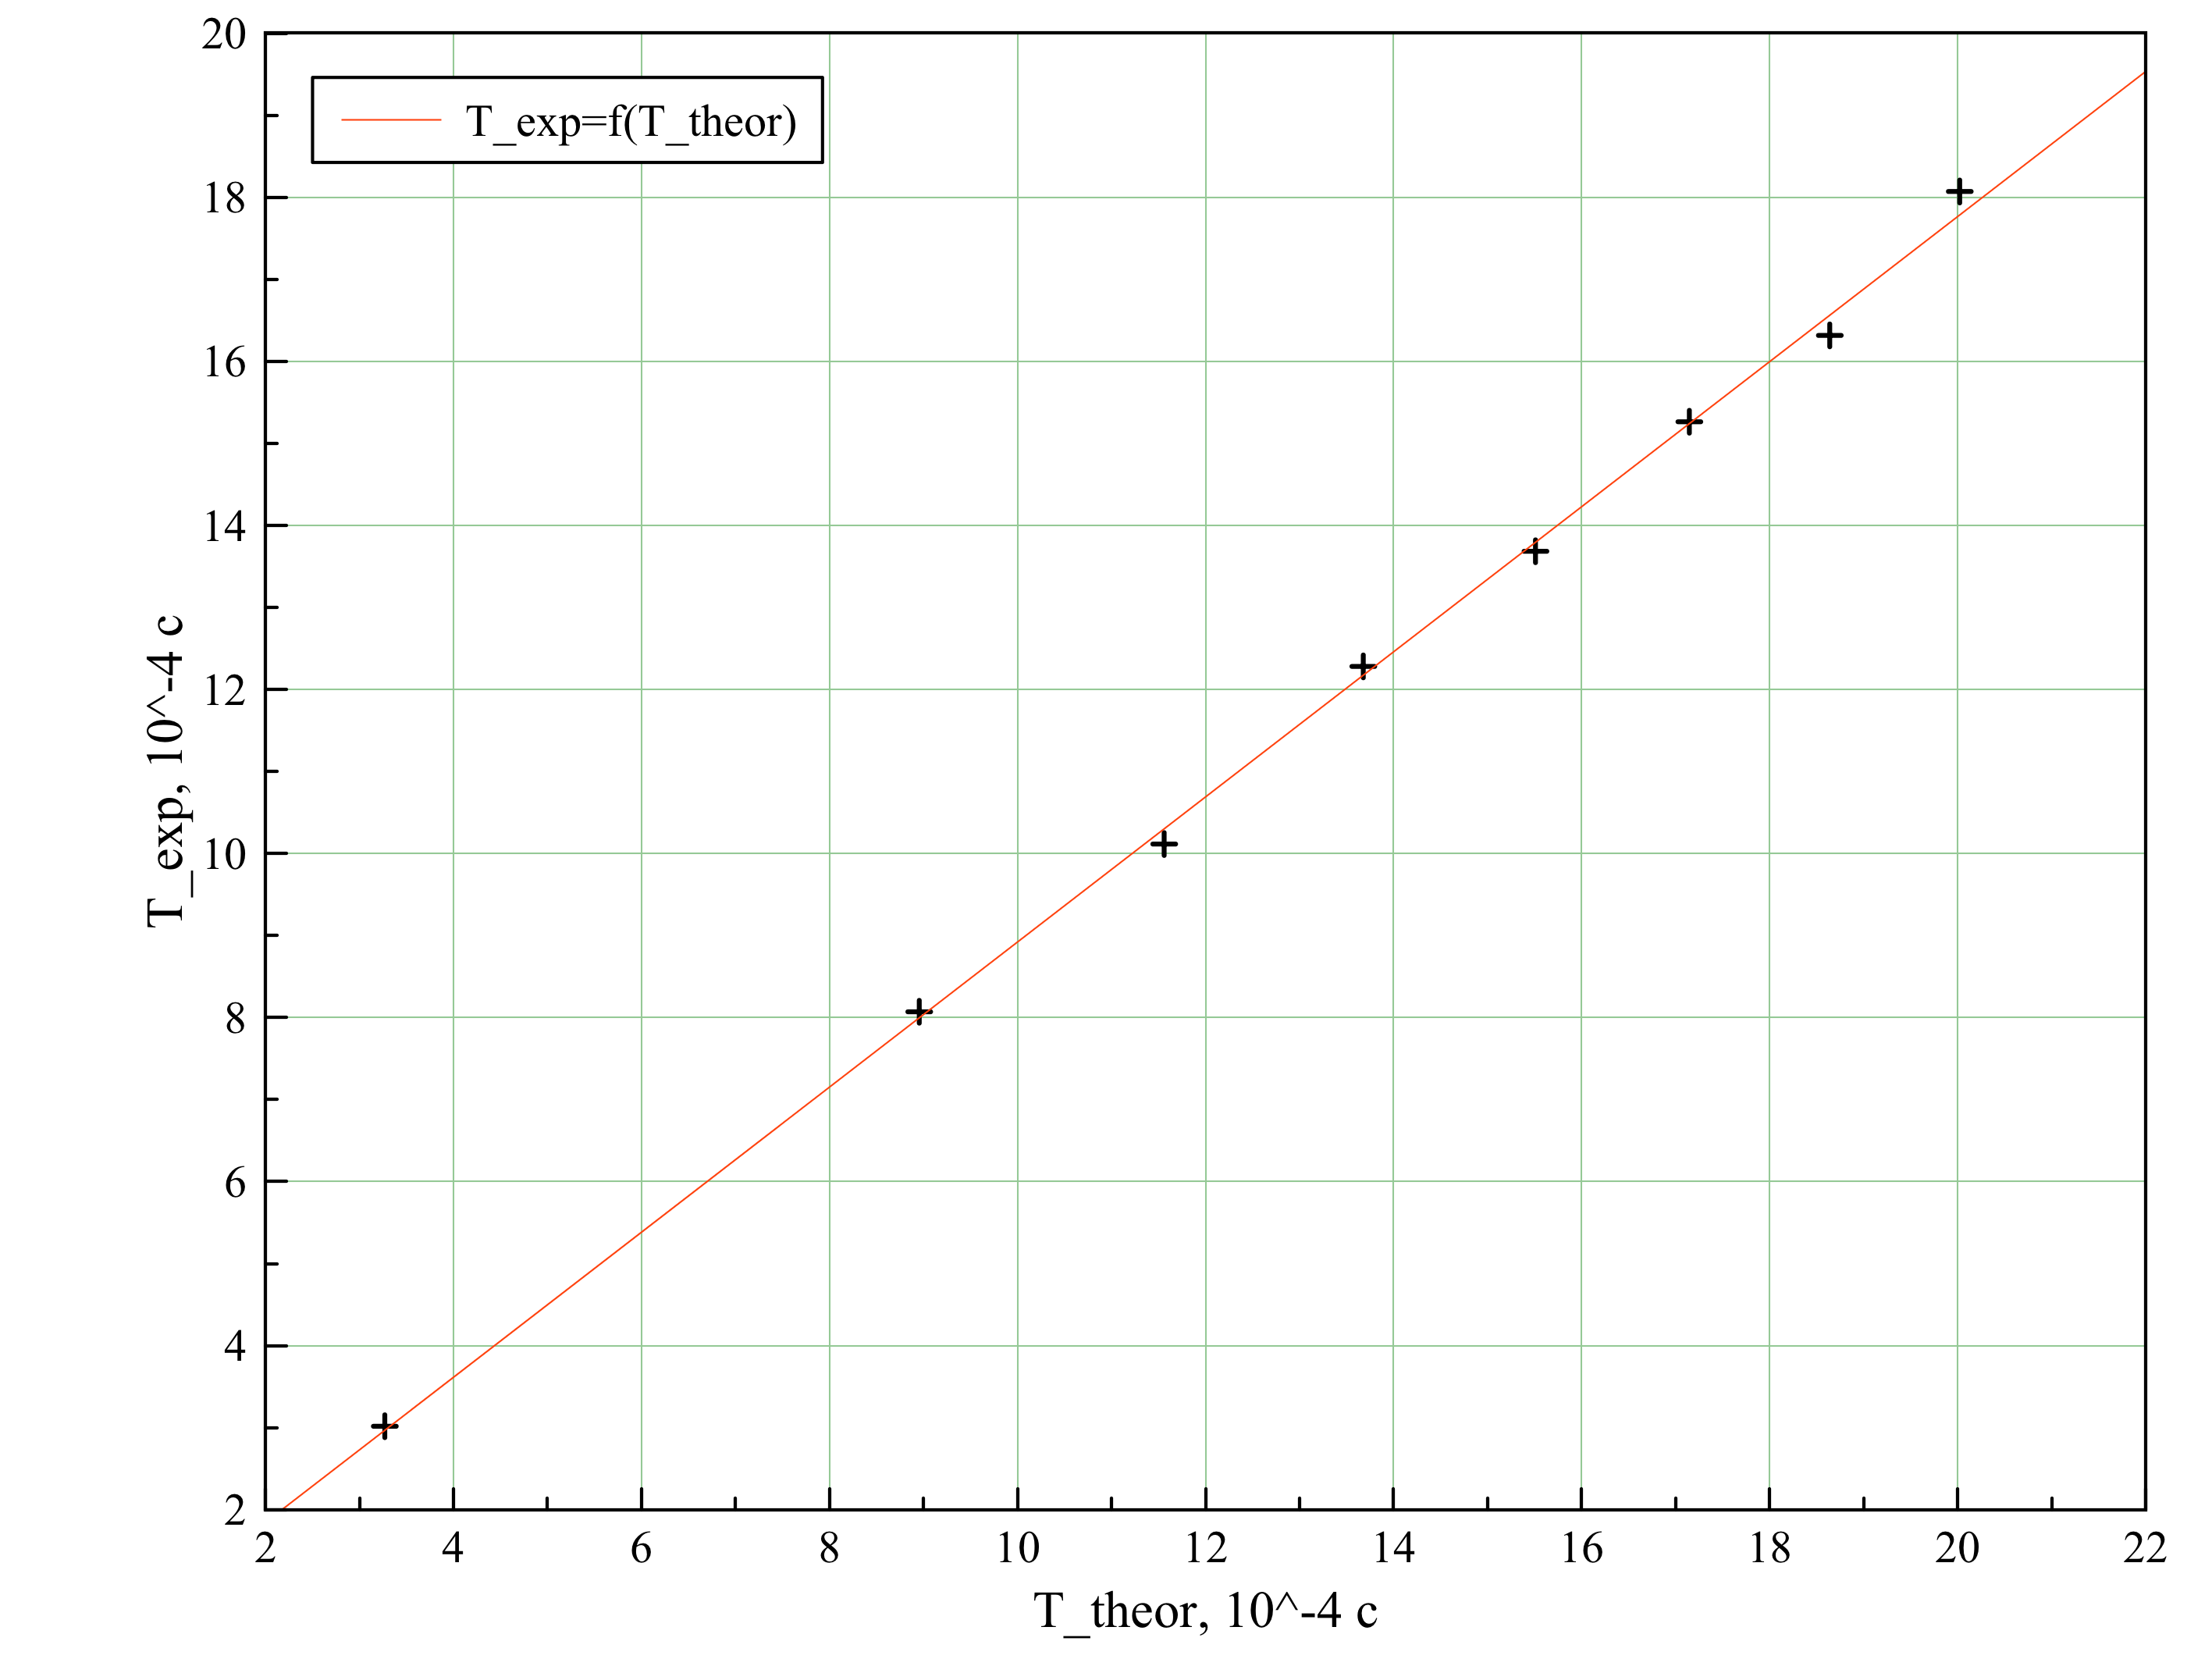
\includegraphics[width=0.8\textwidth]{plot1.png}
	\end{center}
	\end {figure}
	
	\item Приняв $L=200$мГн, рассчитаем емкость $C$, при которой собственная частота колебаний контура $\nu_0 = \cfrac{1}{2\pi\sqrt{LC}}$ равна $5$кГц: $\boxed{C = \cfrac{1}{L(2\pi \nu_0)^2}= 5.07\text{нФ}}$
	Также рассчитаем критическое сопротивление контура для выбранных $L$ и $C$: $\boxed{R_{\text{кр}}^{theor} = 2\sqrt{\cfrac{L}{C}}=12561,5 \text{Ом}}$
	
	\item Экспериментально найдем критическое сопротивление $\boxed{R_{\text{кр}} = 9200 \text{Ом}}$; 
	$R_\text{конт} = R+ R_L$, где $R_L = (14 \pm 1)\text{ Ом}$. 
	Снимем зависимость логарифмического декремента затухания от сопротивления: $$\Theta = \cfrac{1}{n}\ln{\cfrac{U_k}{U_{k+n}}}$$.
	Результаты заносим в Таблицу 2.
		\begin{table}[H]
			\centering
			\begin{tabular}{|c|c|c|c|c|c|c|c|}
				\hline
				$R, \text{ Ом}$ & $R_{\text{конт}}, \text{ Ом}$ & $U_k$ & $U_{k+n}$ & $n$ & $\Theta$ &$1/R_{\text{конт}}^2,  10^{-7}\text{ Ом}^{-2}$& $1/\Theta^2$\\ \hline
				1000     & 1135   & 3.4      & 0.2     & 4         & 0.71         &    9,73  &   1,98               \\ \hline
				1200     &  1335  & 2.9      & 0.1     & 4         & 0.84        &    6,79   &    1,42            \\ \hline
				1500     &  1635  & 2.25      & 0.1     & 3         & 1.04        &   4,36    &    0,92        \\ \hline
				1800     &  1935  & 2.0      & 0.2     & 2         & 1.15        &    3,04   &      0,76         \\ \hline
				2100     &  2235  & 4.1       & 0.2     & 2         & 1.51       &   2,24   &    0,44            \\ \hline
				2400     &  2535  & 3.2      & 0.1     & 2         & 1.73       &    1,72   &    0,33              \\ \hline
			\end{tabular}
			\caption{$1/R^2_{\text{конт}}$ и $1/\Theta^2$}
		\end{table}
		Ошибки измерений: $\sigma_{1/R^2} = \cfrac{1}{R_{\text{конт}}^2}\cfrac{1}{14}$;  $\sigma_{1/\Theta^2} = \cfrac{1}{\Theta^2}\sqrt{\left(\cfrac{\sigma_{U_k}}{U_k}\right)^2+\left(\cfrac{\sigma_{U_{k+n}}}{U_k+n}\right)^2}$\\ 
		Построим график $\cfrac{1}{\Theta^2}=f\left(\cfrac{1}{R_{\text{конт}}}\right)$
		
		\begin {figure}[H]
		\begin{center}
			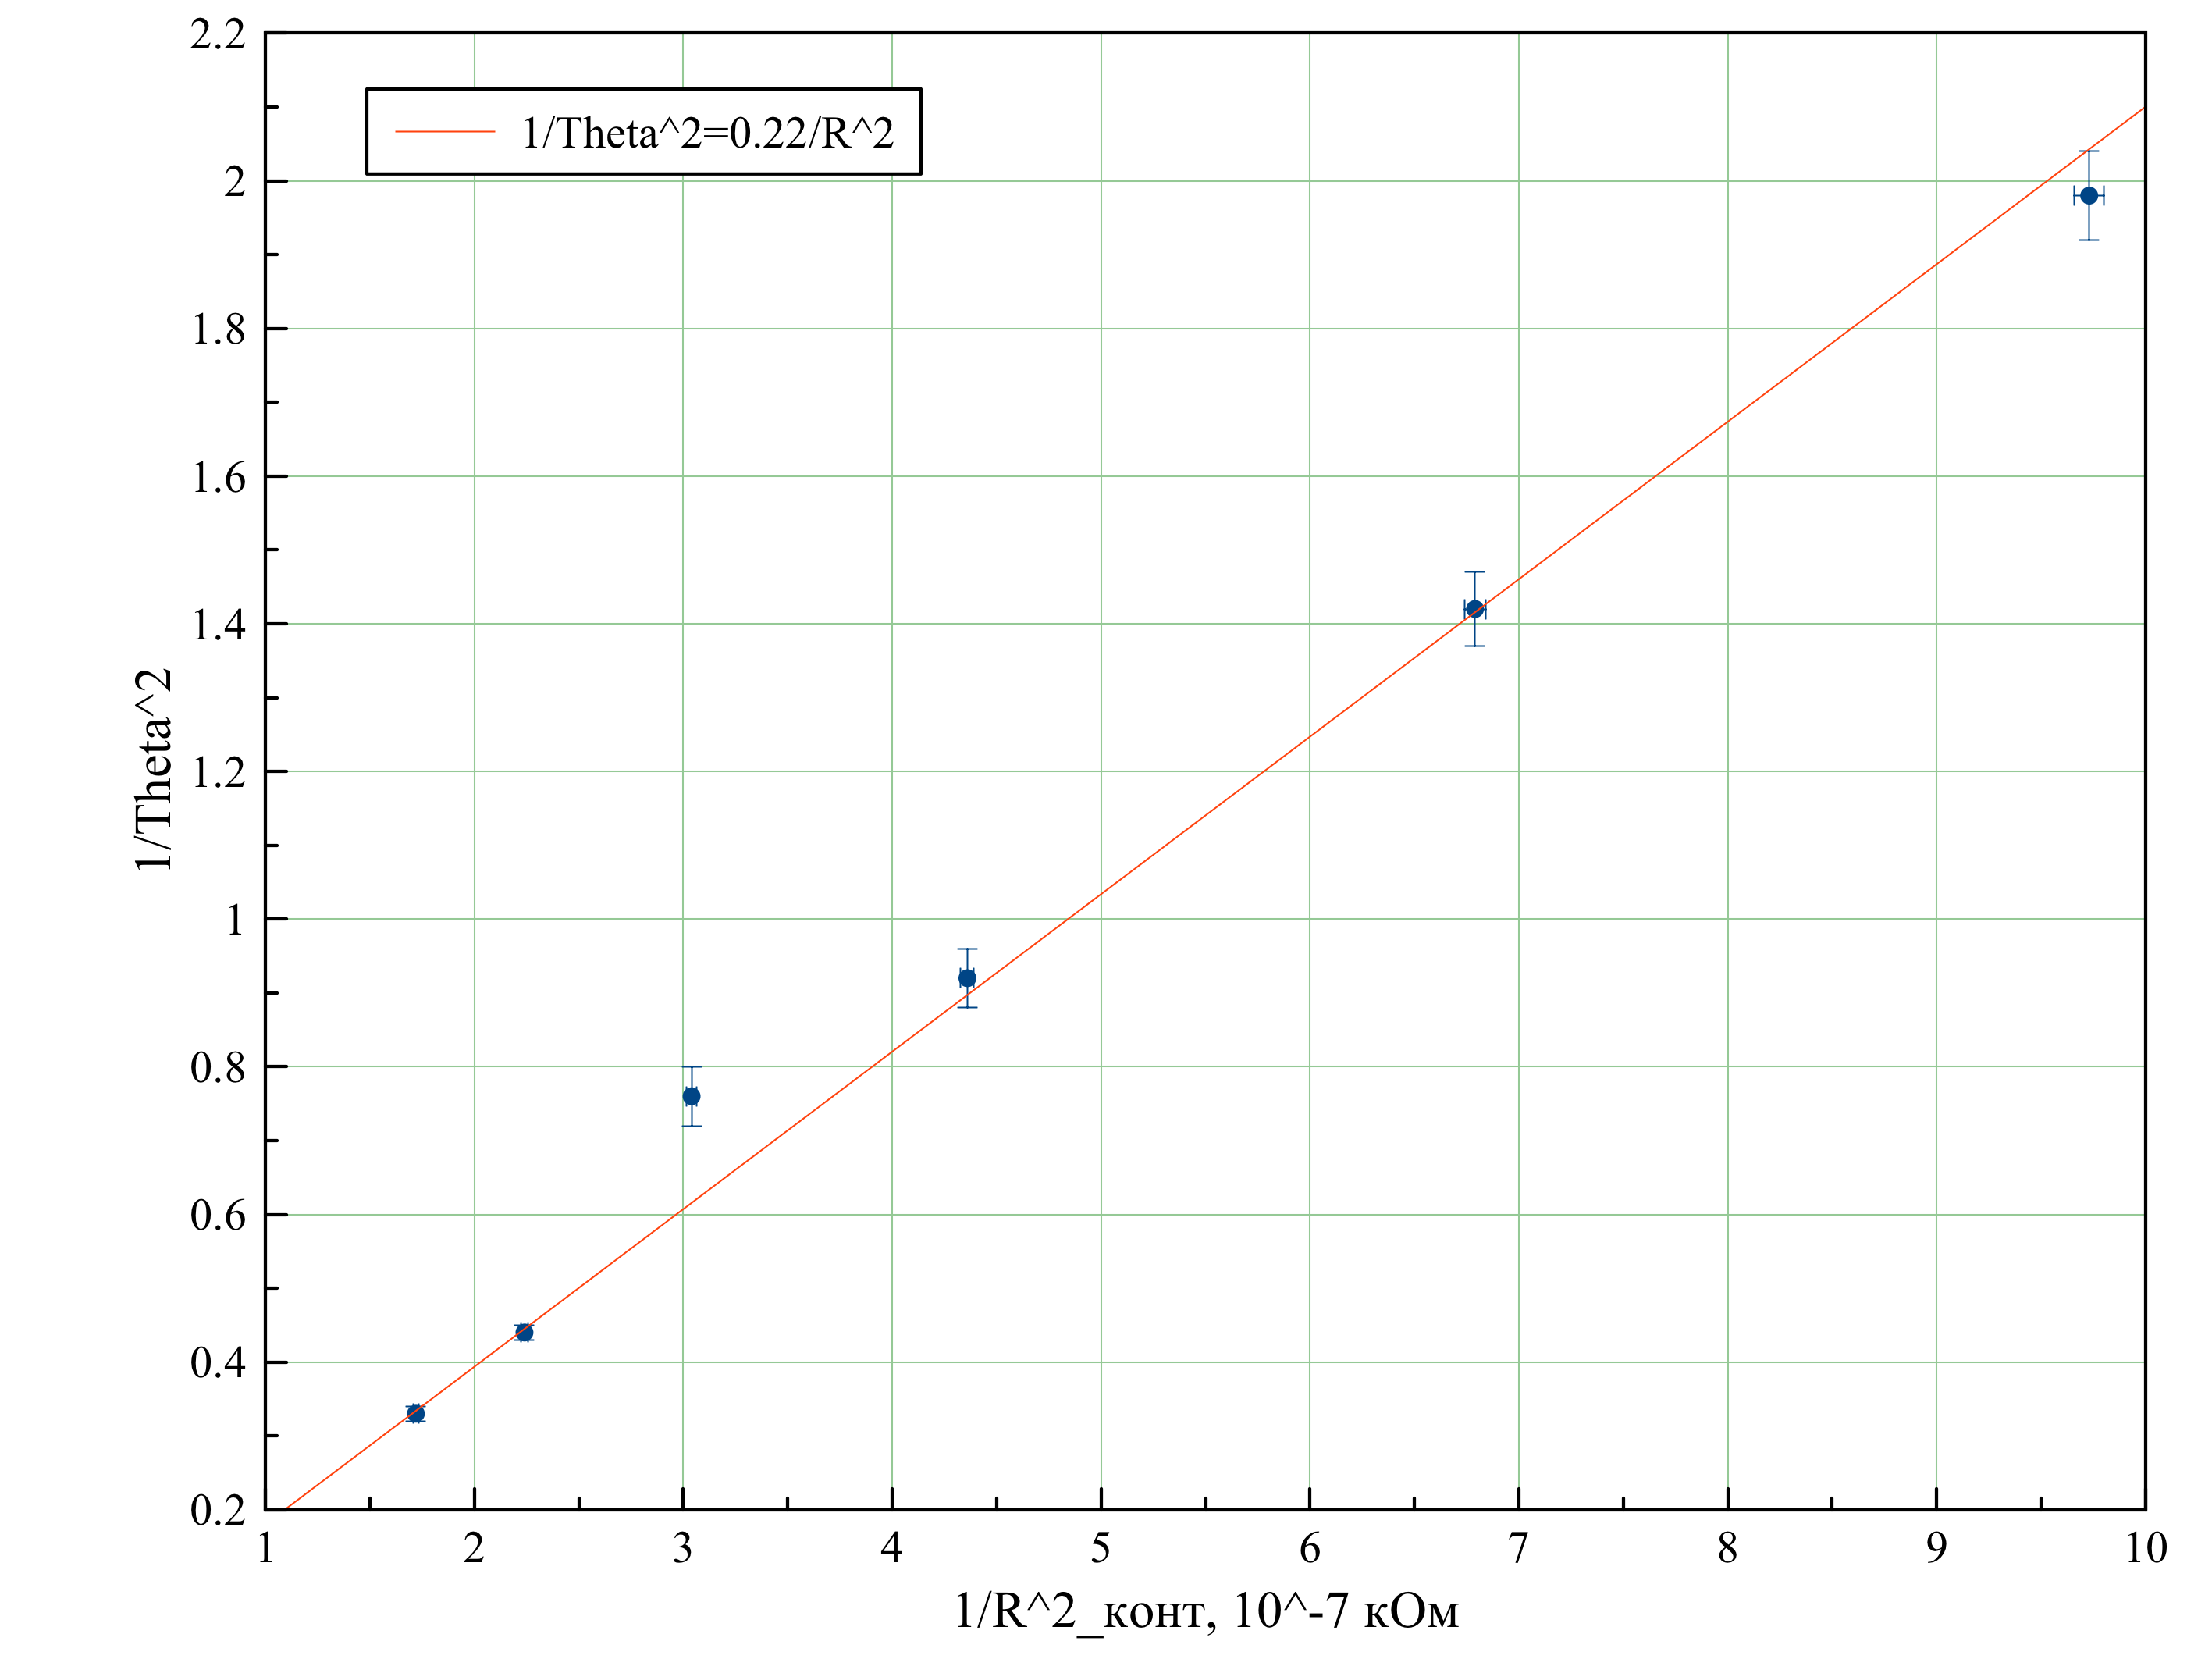
\includegraphics[width=0.8\textwidth]{plot2.png}
		\end{center}
		\end {figure}
		Определим угол наколна графика:
		
		Приняв $Y = \cfrac{1}{\Theta^2}$; $X = \cfrac{1}{R_{\text{конт}}^2}$, получим $R_{\text{крит}} = 2\pi\sqrt{\cfrac{\Delta Y}{\Delta X}}$. В итоге получаем: 
		$$\boxed{R_{\text{крит}}^{graph} = 9.32 \text{ кОм}}$$
		\newpage
	\item Рассчитаем добротность контура для максимального и минимального значений $\Theta$: $Q=\cfrac{\pi}{\Theta}$ и сравним с расчетом $Q$ через параметры контура $R, L, C$: $Q=\cfrac{1}{R}\sqrt{\cfrac{L}{C}}$
	\begin{itemize}
		\item $\Theta_1 = 0.71$, $Q_{\Theta_1} = \cfrac{\pi}{\Theta_1} = 4.42$, $Q_{RLC_1} = \cfrac{1}{R_1}\sqrt{\cfrac{L}{C}}=5.2$
		\item $\Theta_2 = 1.73$, $Q_{\Theta_2} = \cfrac{\pi}{\Theta_2} = 1.82$, $Q_{RLC_2} = \cfrac{1}{R_2}\sqrt{\cfrac{L}{C}}=2.15$
	\end{itemize}
	
	\item Рассчитаем $\Theta$ по спирали
		\begin{table}[H]
			\centering
			\begin{tabular}{|c|c|c|c|c|}
				\hline
				$R, \text{ Ом}$ & $r_{k+n}$ & $r_{k}$ & $n$ & $\Theta$ \\ \hline
				900            & 0.2   & 2.7      & 4    & 0.65                                         \\ \hline
				1000            & 0.1   & 2.2       & 4     & 0.77                                    \\ \hline
				1500          & 0.2   & 4       & 3     & 1                              \\ \hline
				2100             & 0.2   & 3.5       & 2     & 1.43                                      \\ \hline
				2300             & 0.2   & 3.6       & 2     & 1.45                             \\ \hline
			\end{tabular}
			\caption{расчет по спирали}
		\end{table}
\end{enumerate}



\section{Вывод}
В данной работе исследовали зависимость периода свободных колебаний контура от емкости, зависимость логарифмического декремента от сопротивления, а также определили критическое сопротивление разными способами и добротность контура. Все три значения критического сопротивления достаточно близки по значению за исключением рассчитанного теоретически. Данное значение достаточно сильно отклонилось от двух других вследствие того, что мы принимали L примерным, не рассчитывали его точно. В двух других измерениях: экспериментальном и по графику -- никаких значений наугад не брали. Также расчет добротности и логарифмического декремента (расчеты прямые и по спирали) разными способами дали примерно одни и те же значения.


\end{document}